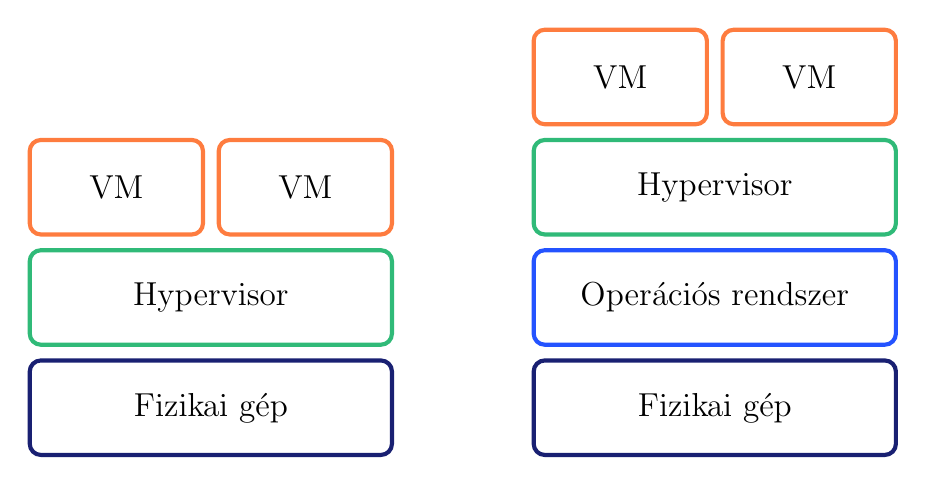
\begin{tikzpicture}[node distance=1.4cm]
	\definecolor{midnightblue}{HTML}{192072}
	\definecolor{junglegreen}{HTML}{30BA78}
	\definecolor{waterholeblue}{HTML}{2453FF}
	\definecolor{persimmon}{HTML}{FE7C3F}

	\tikzstyle{rect} = [rectangle, rounded corners, draw=midnightblue, minimum width=4.6cm, minimum height=1.2cm, text centered, text=black, font=\fontsize{12}{12}\selectfont, line width=1.5pt]
	\tikzstyle{vm-rect} = [rectangle, rounded corners, draw, minimum width= 2.2cm, minimum height=1.2cm, text centered, font=\fontsize{12}{12}\selectfont, line width=1.5pt]
	
	\node (hardware) [rect] {Fizikai gép};
	\node (hypervisor) [rect, above of = hardware, draw=junglegreen] {Hypervisor};
	\node (vm1) [vm-rect, above of = hypervisor, xshift=-1.2cm, draw=persimmon] {VM};
	\node (vm2) [vm-rect, above of = hypervisor, xshift=1.2cm, draw=persimmon] {VM};

	\node (hardware2) [rect, right of = hardware, xshift=5cm] {Fizikai gép};
	\node (os) [rect, above of = hardware2, draw=waterholeblue] {Operációs rendszer};
	\node (hypervisor2) [rect, above of = os, draw=junglegreen] {Hypervisor};
	\node (vm1_2) [vm-rect, above of = hypervisor2, xshift=-1.2cm, draw=persimmon] {VM};
	\node (vm2_2) [vm-rect, above of = hypervisor2, xshift=1.2cm, draw=persimmon] {VM};

\end{tikzpicture}
